\chapter[Metodologia]{Metodologia}


\section{Proposta Geral}
Ao analisar a história de mixers e equipamentos e o mercado atual, chega-se a conclusão de que a evolução dos equipamentos foi e é realizada partindo de um modelo que se baseia na mixagem feita em vinil. Ao longo do tempo, acrescentou-se novas funcionalidades e formas de interações, porém, na maioria das vezes, mantendo o jogger para atraso e avanço da música, \textit{fadder} para volume e knobs para frequências.
\par
Além disso, conforme a evolução da microeletrônica, equipamentos começaram a migrar aos poucos para a eletrônica digital, culminando na utilização de um DSP para o processamento do sinal de áudio para comportar formatos de música com baixa compressão como WAV e FLAC. 
\par
Assim, o que se vê hoje são dois extremos: equipamentos extremamente caros mas que não necessitam da presença de um computador e equipamentos dependentes, que são mais baratos e acabam possuindo melhor qualidade nos processamentos, que dificultam a mobilidade.
\par
Além disso, em experiência adquiridas com \textit{DJs}, observa-se que uma das maiores dificuldades que iniciantes possuem é realizar um ajuste fino entre as bandas de frequências quando lidam com \textit{mixers} clássicos de ajustes de três bandas. E é essa habilidade que permite o artista de destacar elementos de músicas e criar uma nova atmosfera. Apesar disso, quando o estilo de gênero de um \textit{DJ} está consolidad em uma área, a mixagem se torna mais mecânica, de forma que os elementos entre as música selecionadas se tornam semelhantes, o que permite maior flexibilidade na alteração de parâmetros de mixagem. Ou seja, há menos margem para que uma colagem sonora feita se torne desagradável aos ouvidos.
\par
Dessa forma, o intuito é conceber um \textit{mixer} que conte com um controle central, que visa controlar duas músicas, ou dois \textit{decks}. Em contrapartida à estrutura clássica de mixagem, que conta com controles de ganho de três bandas de frequência para cada canal, a proposta visa a utilização de um filtro passa-altas para cada canal. 
\par
O dispostivo conta com dois canais de entrada, ou seja, duas músicas de entrada. Conforme um filtro está passando toda a banda de um canal, o outro filtro automaticamente está rejeitando o outro canal. E conforme o controle central avança em direção ao canal dois, a frequência de corte do primeiro canal aumenta, diminuindo a presença da música um, enquanto a frequência de corte do canal dois diminui, aumentando a presença de elementos da música dois. 
\par
Assim, um controle central de frequência comanda ambas frequências de corte. Quando esse controle está em um extremo, apenas um canal é transmitido para a saída. Já no outro extremo, apenas o outro canal é transmitido. E conforme o controle avança de um extremo a outro, uma combinação entre as duas músicas é transmitida à saída.
\par
Alguns equipamentos atuais contam com ferramentas de mixagem automática, na qualuma lista de músicas é selecionada. O próprio sistema realiza a sincronia de tons e a transição entre um canal e outro, através de um sistema de \textit{fader}, no qual o volume de um canal é atenuado, enquanto o do outro obtém um ganho, até que a transição seja finalizada.
\par
Porém, esse tipo de sistema não leva em conta nuances da música ou qual seria o melhor momento para que a entrada da próxima música aconteça.
\par
Assim, o sistema proposto permite ao artista uma mixagem mais simples, sem grandes preocupações acerca do controle de bandas de frequência; modelo que pode facilitar mixagem para artistas que possuem uma biblioteca similar e consolidada ou jovens artistas que ainda não possuem total controle sobre as bandas de frequência mas que queiram experimentar.
\par
Para além de uma mixagem mais simples, o sistema propõe o uso de efeitos para que o artista tenha mais liberdade durante a criação de sua mixagem. Dessa forma, o sistema conta com a presença de dois efeitos: \textit{delay} e \textit{reverb}, que podem funcionar de forma automática; também controlada pelo botão central.
\par
A lógica de funcionamento do efeito leva em consideração a posição do botão central, já que quando o mesmo se encontra em uma posição na qual duas músicas estão sendo tocadas, entende-se que uma transição está acontecendo. Dessa forma, de forma automatizada, a presença do efeito parte do nulo até alcançar o seu máximo (na posição do meio do botão central) e conforme a posição do botão vai a uma extremidade, a presença do efeito diminui, pois se considera que a transição já foi realizada.
\par
Portanto, a proposta deste projeto visa implementar um sistema que leia dois sinais analógicos, correspondentes a sinais músicais advindo de toca-discos, CDJs ou qualquer equipamento que transmita sinais de áudio analógicos. Esses sinais serão processados em tempo real a partir de filtros passa-altas que são controlados por um botão central. Além disso, o sistema deve permitir ao usuário a possibilidade de selecionar qual efeito ele deseja utilizar, de forma que se selecione a quantidade da presença do efeito, possibilitando ao usuário rejeitar a presença do efeito quando a presença for nula.
\par
A implementação visa utilizar botões \textit{sliders} para o controle central e presença de efeitos e um botão \textit{on}/\textit{off} para a seleção do efeito. 

\section{Levantamento de Requisitos}

O levantamento de requisitos é uma etapa crucial no desenvolvimento de qualquer sistema, pois define as funcionalidades e características que ele deve possuir para atender às necessidades dos usuários finais. Nesta seção, são apresentados os requisitos funcionais e não funcionais, que especificam o comportamento esperado do sistema, assim como as restrições e qualidades que devem ser atendidas. Os requisitos foram organizados em categorias que abrangem desde aspectos de desempenho e interface do usuário até segurança e manutenção, assegurando uma visão completa e detalhada do que o sistema deve entrega

\subsection{Requisitos Funcionais}
\begin{itemize}
    \item O sistema deve permitir ao \textit{DJ} utilizar tanto CDJs quanto toca-discos.
    \item O sistema deve permitir ao \textit{DJ} controlar a presença dos dois canais.
    \item O sistema deve permitir ao \textit{DJ} controlar a presença dos efeitos.
\end{itemize}

\subsection{Requisitos Não Funcionais}
\begin{itemize}
    \item O sistema deve responder aos comandos do \textit{DJ} com latência mínima, garantindo uma experiência de mixagem fluida.
    \item A interface do usuário deve ser intuitiva e fácil de usar, permitindo que o \textit{DJ} faça ajustes rapidamente durante a performance.
    \item O sistema deve ser confiável e estável, capaz de lidar com longos períodos de uso contínuo sem falhas.
    \item O sistema deve oferecer uma qualidade de som de alta fidelidade, garantindo que o áudio reproduzido seja claro e com mínimas distorções.
\end{itemize}

\subsection{Requisitos de Interface do Usuário}
\begin{itemize}
    \item A interface do mixer deve incluir botões físicos ou controles táteis para ajuste de frequência e efeitos de áudio.
    \item A interface do mixer deve ser organizada de forma lógica e intuitiva, com controles agrupados por função para facilitar a navegação.
    \item A interface deve possuir indicações das funções dos botões de interação com o usuário.
\end{itemize}

\subsection{Requisitos de Sistema}
\begin{itemize}
    \item O sistema deve ser compatível com uma variedade de dispositivos de áudio externos, como CDJs e toca-discos.
    \item O sistema deve ser alimentado por uma fonte de energia padrão, como uma tomada elétrica.
    \item O sistema deve incluir interfaces de entrada e saída de áudio padrão RCA.
\end{itemize}

\subsection{Requisitos de Desempenho}
\begin{itemize}
    \item O sistema deve ser capaz de lidar com até dois canais de áudio simultaneamente, sem comprometer a qualidade do som ou a responsividade dos controles.
    \item O sistema deve suportar uma ampla gama de frequências de áudio, garantindo que os graves sejam reproduzidos com graves e os agudos sejam nítidos e claros.
\end{itemize}

\subsection{Requisitos de Segurança}
\begin{itemize}
    \item O sistema deve ser projetado para minimizar o risco de danos aos equipamentos de áudio conectados, oferecendo proteção contra sobrecarga ou curto-circuito.
\end{itemize}

\subsection{Requisitos de Manutenção}
\begin{itemize}
    \item O sistema deve ser projetado para facilitar a manutenção e reparo, com acesso fácil aos componentes internos e documentação clara sobre procedimentos de serviço.
\end{itemize}

\subsection{Requisitos de Compatibilidade}
\begin{itemize}
    \item O sistema deve ser capaz de se comunicar perfeitamente com qualquer dispositivo de reprodução de música profissional como canal de entrada e qualquer sistema de som de sáida. 
\end{itemize}

\newpage
\section{Fluxograma do Mixer}

O \textit{mixer} proposto possui subblocos de funcionamento e se interligam conforme se encontra na Figura \ref{fig52}.

De forma geral, o sistema funciona em um laço contínuo de leitura de sinais, tanto das músicas quanto dos controles, e modificações de parâmetros para que os sinais sejam processados, e, enfim, reproduzidos. Assim, cada ciclo pode ser representado na Fig. \ref{fig52}.

\begin{figure}[h]
    \centering
    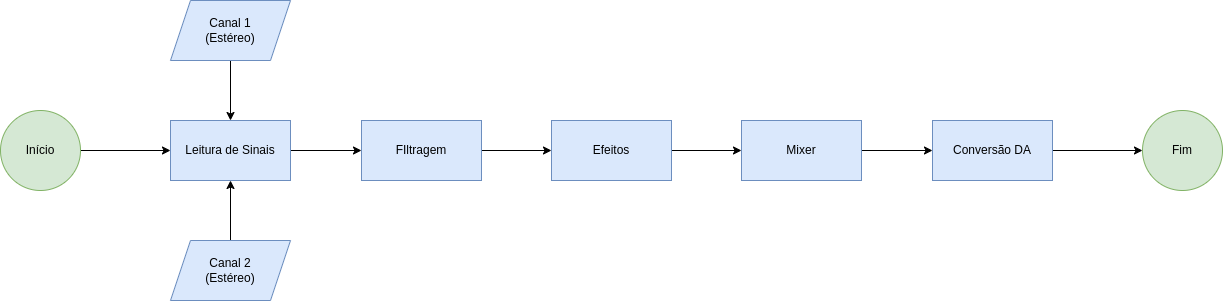
\includegraphics[width=\textwidth]{figuras/fig52.png}
    \caption{fluxograma geral do \textit{mixer}}
    \label{fig52}
\end{figure}

Assim, a partir dos dispositivos de reprodução de música, os sinais adentrarão o sistema, de forma que serão convertidos para sinais digitas. Enquanto isso, é feita uma varredura dos valores correntes dos controles disponíveis na interface.

Conforme se adquire valores para os parâmetros, tanto a filtragem de sinais quanto o processamento dos efeitos são realizados novamente a fim de ajustarem seu comportamento conforme os novos valores dos controles.


Por fim, os sinais da filtragem e do efeito são combinados e convertidos para analógico, de forma que possam ser reproduzidos ao final.

Nas subseções abaixo, cada bloco presente no Fluxograma Geral do Sistema, Fig. \ref{fig52}, será detalhado sobre o seu funcionamento conceitual proposto através de um subfluxograma, que detalha o processamento interno.

\subsection{Bloco de Conversão AD}
Esse bloco é responsável pela aquisição e conversão dos sinais analógicos em sinais codificados. Esses sinais são tanto obtidos pelo reprodutor de música, seja uma CDJ, um toca-discos, quanto pelos botões de controle, presentes na interface do usuário.

\begin{figure}[h]
    \centering
    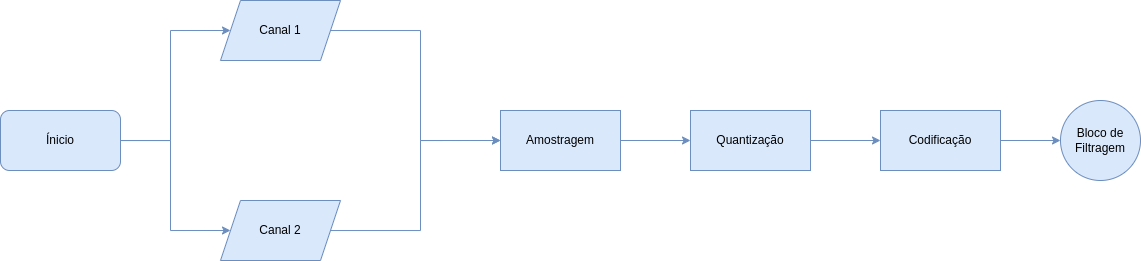
\includegraphics[width=\textwidth]{figuras/fig53.png}
    \caption{bloco de conversão analógico digital}
    \label{fig53}
\end{figure}

As entradas desse bloco são os sinais analógicos e a saída são os sinais digitais. Dessa forma, os processos que devem ser realizados nesses sinais incluem amostragem, quantização e codificação, para que, enfim, o sinal possa ser lido pela unidade de processamento.

\subsection{Bloco de Leitura de Sinais}

Os sinais analógicos que são lidos incluem os sinais de música; e os sinais de controle que são advindos de dois potenciômetros e de um botão de duas posições, respectivamente para obtenção da frequência central, da quantidade de efeito desejado presente no processamento e o de escolha de qual efeito se deseja utilizar. 


\begin{figure}[h]
    \centering
    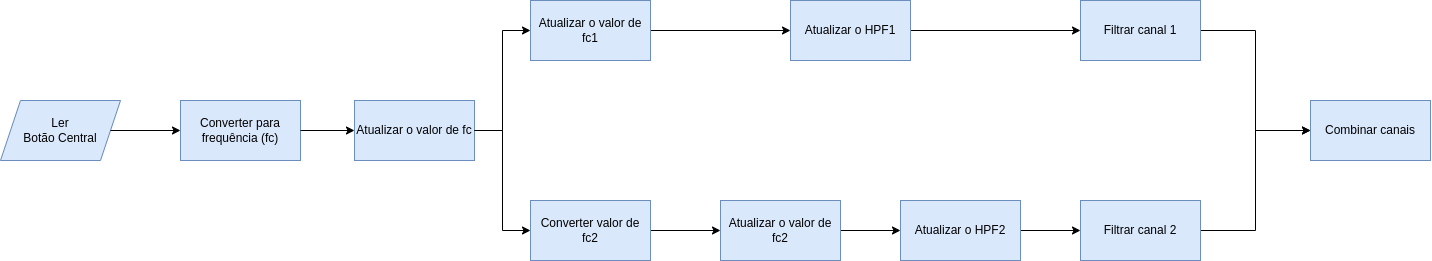
\includegraphics[width=\textwidth]{figuras/fig54.png}
    \caption{bloco de leitura de sinais analógicos}
    \label{fig54}
\end{figure}

As operações realizadas nesses sinais são visualizados na Figura \ref{fig54}.

\subsection{Bloco de Filtragem}

No bloco de filtragem, os sinais já estão no domínio digital. Assim, deve-se ler a posição do botão central. Esse sinal é adquirido através da conversão de um sinal analógico advindo de um potenciômetro e convertido, de um sinal elétrico para um digital. 

Assim, pode-se obter a posição na qual o botão se encontra. Essa posição, que se encontrará em um intervalo de valores quantizados, será normalizado e convertido para um valor de frequência de corte, ou seja, estará entre 20 e 22050 Hz.

Com esse valor de frequência de corte, o filtro passa-altas do canal 1 será atualizado; e seu sinal filtrado. 

No canal 2, um novo valor para a frequênca de corte 2 será obtido através da expressão de Equação \ref{eq:05}. Assim, o filtro passa-altas deste canal será atualizado conforme a nova frequência de corte, como se encontra na Figura \ref{fig55}. 

No bloco de filtragem, todos os sinais analógicos já estão codificados de forma que podem ser processados digitalmente. Assim, tem-se a \textit{fc} como o valor de frequência entre 20 a 22050 Hz. Dessa forma, valores são atribuídos aos parâmetros \textit{fc$_{1}$} e \textit{fc$_{2}$}.

\begin{figure}[h]
    \centering
    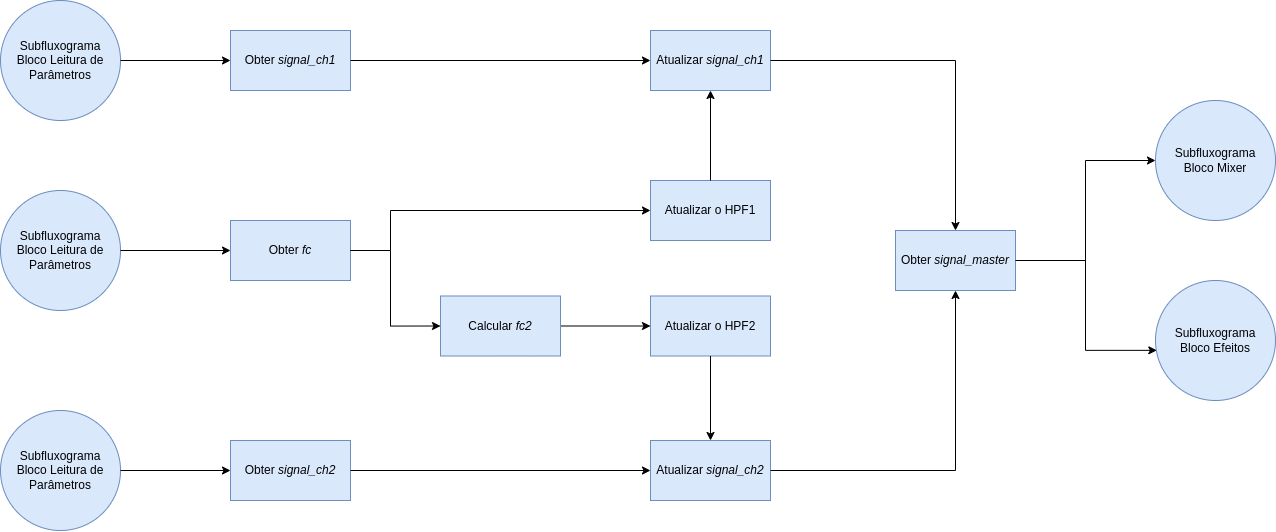
\includegraphics[width=\textwidth]{figuras/fig55.png}
    \caption{bloco de filtragem}
    \label{fig55}
\end{figure}

No subfluxograma da Figura \ref{fig55}, \textit{fc} corresponde à frequência de corte central, ou seja, àquela lida e convertida do botão central; \textit{fc$_{1}$} é a frequência de corte para o filtro passa-altas 1 (HPF1) e \textit{fc$_{2}$} é a frequência de corte do canal 2 para o filtro passa-altas 2 (HPF2).

Ao final, os dois canais são combinados e se tem o sinal \textit{signal\_master}, que é mandado tanto para o bloco de processamento de efeitos quanto o bloco final de combinação dos dois sinais: de efeito e de combinação dos canais 1 e 2.

\subsection{Bloco de Efeitos}

Os efeitos do \textit{mixer} podem ter seus parâmetros de quantidade de reverberação após 1s e o intervalo de atraso (em milissegundos) de amostras configurados conforme o botão de quantidade de efeito. 

\begin{figure}[h]
    \centering
    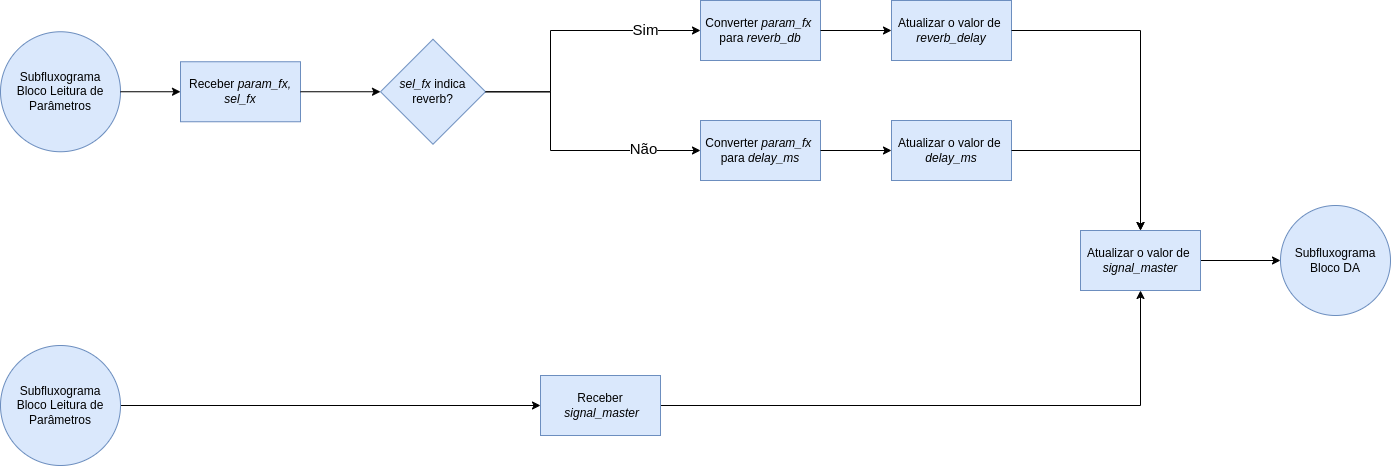
\includegraphics[width=\textwidth]{figuras/fig56.png}
    \caption{bloco de efeitos}
    \label{fig56}
\end{figure}

Além disso, o usuário poderá escolher qual efeito deseja utilizar através de um botão de duas posições, conforme a Figura \ref{fig56}. Os dois parâmetros de seleção e quantidade de efeitos são obtidos do bloco de leitura de sinais. Ao fim desse bloco, tem-se o sinal isolado do efeito, ou seja, o sinal obtido ao final do bloco \textit{mixer} com o efeito aplicado, atribuído ao \textit{signal\_fx}. 

\subsection{Bloco de Automação de Efeitos}

Nesse \textit{mixer} proposto, o volume do efeito é ajustado automaticamente, conforme a frequência central presente na Figura \ref{fig57}. Assim, quando a \textit{fc} está nas extremidades, o volume do efeito é nulo. Porém, ele obtém um ganho conforme a \textit{fc} alcança a posição central da banda de frequênca.

\begin{figure}[h]
    \centering
    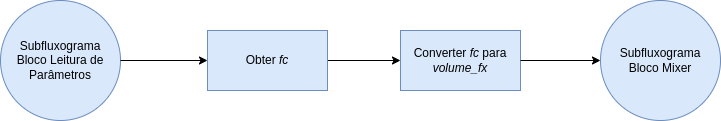
\includegraphics[width=\textwidth]{figuras/fig57.png}
    \caption{bloco de automação do volume de efeitos}
    \label{fig57}
\end{figure}

Para a obtenção do ganho do efeito, uma expressão é utilizada para a conversão do valor da \textit{fc} em \textit{volume\_fx}, que é o ganho do \textit{signal\_fx}.


\subsection{Bloco Mixer}

A operação de somar dois sinais recebe o nome de \textit{mixing}. Dessa forma, entende-se que nesse processo há dois momentos em que os sinais são misturados. O primeiro é quando os sinais dos canais 1 e 2 são misturados. Outro momento acontece quando os sinais já misturados dos canais 1 e 2 são misturados com o sinal do efeito. Nesse caso, esse bloco se refere à mistura final, ou seja, do segundo caso.

    \begin{figure}[h]
        \centering
        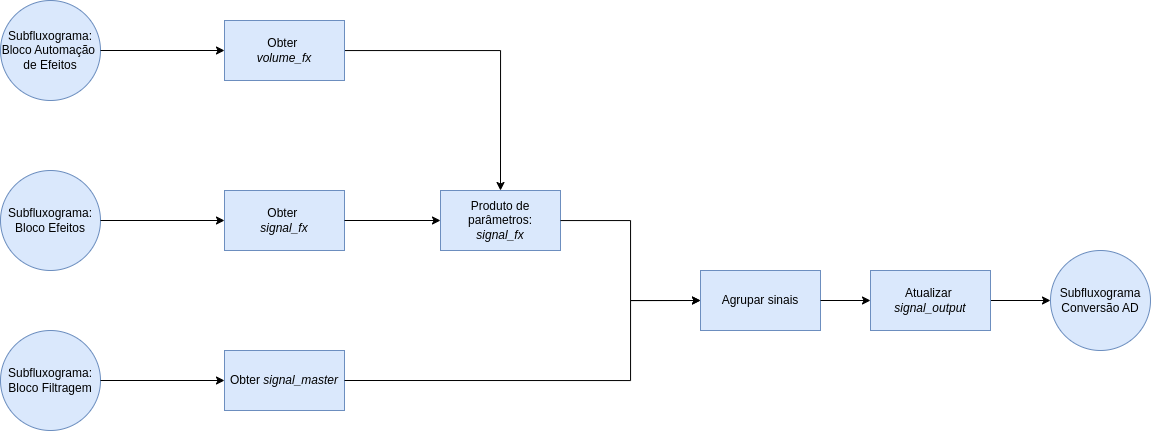
\includegraphics[width=\textwidth]{figuras/fig58.png}
        \caption{bloco de mistura final de sinais}
        \label{fig58}
    \end{figure}

No subfluxograma da Figura \ref{fig58}, o sinal do efeito é atenuado ou amplificado conforme o volume obtido pelo bloco de automação de volume de efeitos. Assim, esse sinal de efeito com volume ajustado é misturado com o sinal obtido do bloco de filtragem, de forma que o sinal de saída, \textit{signal\_output}, é obtido. Porém, esse sinal ainda se encontra no domínio digital.


\subsection{Bloco de Conversão AD}

O sinal de saída obtido pelo bloco \textit{mixer} precisa ser convertido para um sinal analógico para que possa ser reproduzido em um sistema de som.

    \begin{figure}[h]
        \centering
        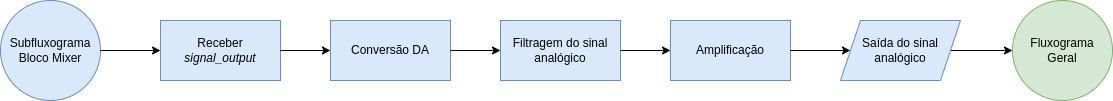
\includegraphics[width=\textwidth]{figuras/fig59.png}
        \caption{bloco de conversão digital analógico}
        \label{fig59}
    \end{figure}

Dessa forma, conforme a Figura \ref{fig59}, o sinal digital passará por processos de conversão digital analógico, filtragem e amplificação da sua potência para que enfim possa ser reproduzido por caixas de som.

\newpage
\section{Prova de Conceito}

Nessa seção, encontra-se uma implementação em um ambiente virtual no qual se pode simular a lógica de funcionamento do sistema.

	\subsection{\textit{PureData}}
    O \textit{PureData} \cite{puredata} é um ambiente de música computacional programável para análise, síntese e processamento de áudio através de sinais digitais em tempo real. 
    

    Esse ambiente permite, através dos seus blocos, a criação de sistemas de processamento de áudio com inúmeras funções implementadas, tanto pelos seus criadores quanto pela sua extensa comundiade. Nele, foi possível a criação de uma prova de conceito que engloba a lógica do botão central com o comando das frequências de corte, bem como o funcionamento dos efeitos. Para simular os sinais de entrada, utilizou-se arquivos WAV locais.

    Assim, a demonstração do sistema se divide em duas grandes funcionalidades: filtragem e efeitos.

	\subsection{Implementação de Filtragem}

    A filtragem lê dois arquivos de música no formato WAV, utilizando as funções \texttt{open}, \texttt{start} e \texttt{stop} para localização, execução e parada da reprodução, respectivamente. Em seguida, utilizou-se o comando \texttt{readsf\textasciitilde\ 2 1e+06} que configura a leitura dos sinais de forma estéreo e utilizando um milhão de amostras no seu \textit{buffer}. O mesmo processo é realizado para ambos arquivos. 

    Em seguida, utilizou-se a função \texttt{hip\textasciitilde}, que corresponde a aplicação de um filtro passa-altas. Porém, neste caso, o argumento que a função utiliza difere entre o canal 1 e 2. Conforme a Figura \ref{fig24}, o canal 1 ("FC do HPF1") recebe diretamente o parâmetro \textit{fc}, advindo do \textit{slider} em azul.
    
    Porém, o filtro passa-altas do canal 2 ("FC do HPF2") recebe um valor ajustado por uma expressão anterior, representada pela Equação \ref{eq:05}. Esse ajuste permite com que uma pequena variação na \textit{fc$_{1}$} promova uma grande variação em \textit{fc$_{2}$} e vice-versa. Além disso, em frequências centrais, a variação entre eles se torna mais similar. Essa expressão coincide com a descrição de um círculo de raio sendo a frequência de amostragem, que é o intervalo do botão central, centralizado no ponto (22050, 22050).

    \begin{equation}  \label{eq:05}
        fc_2 = 22050 - \sqrt{22050^2 - (fc - 22050)^2}
    \end{equation}

    Esse ajuste presente na Equação \ref{eq:05} tem a função de ponderar mudanças nas frequências pois mudanças lineares não são eficientes nesse caso de um controle centralizado, conforme se encontram as frequências de ambos canais na Figura \ref{fig45}.

    \begin{figure}[h]
        \centering
        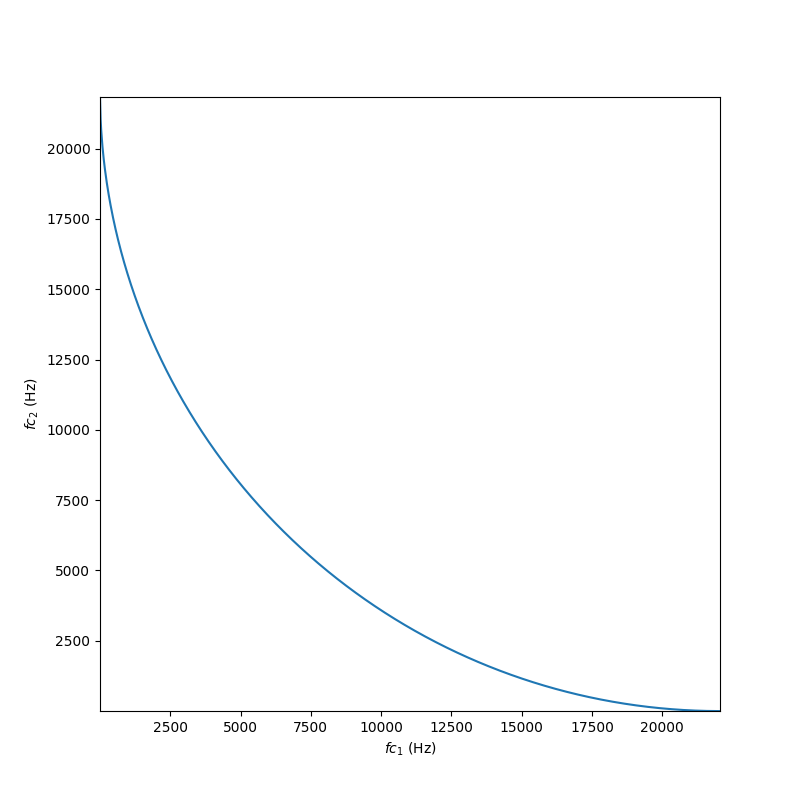
\includegraphics[width=0.7\textwidth]{figuras/fig45.png}
        \caption{expressão para a fc$_{2}$}
        \label{fig45}
    \end{figure}

    \newpage
    Mudanças na casa de centenas no canal 1 causariam pouco efeito no canal 2 pois as baixas frequências possuem maior ganho em relação às altas frequências. Além disso, a mesma lógica pode ser aplicada no outro extremo do controle de frequência. 

    \begin{figure}[h]
        \centering
        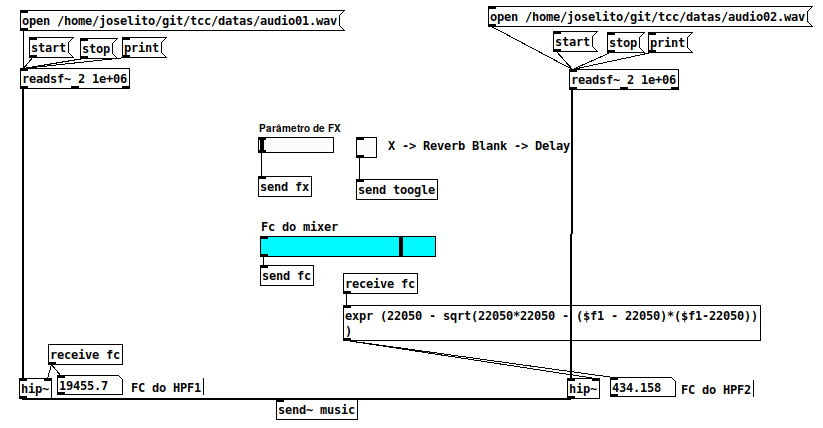
\includegraphics[width=0.9\textwidth]{figuras/fig44.png}
        \caption{lógica de funcionamento do botão central no \textit{PureData}}
        \label{fig44}
    \end{figure}

    Na Figura \ref{fig44}, a frequência obtida do botão central, indicada como \( f_c \), varia de 0.2 a 22050 Hz. A frequência de corte do canal 1, referida como FC do HPF1, é equivalente a \( f_c \) do botão central. A frequência de corte do canal 2, identificada como FC do HPF2, é obtida pela Equação \ref{eq:05}. O sinal resultante, \texttt{send\textasciitilde\ music}, é a soma dos sinais filtrados dos canais 1 e 2.

	\subsection{Implementação de Efeitos}

    O funcionamento do efeito utiliza três parâmetros. Um botão \texttt{toogle}, cuja função é alternar entre os efeitos \textit{delay} e \textit{reverb}; um \textit{slider} que varia parâmetros internos dos efeitos e a frequência de corte do botão central, que automatiza o volume do efeito.

    O botão \texttt{toogle} visa alternar os efeitos. Possui duas posições, ou seja, sempre um efeito está ativo. Para alternar para o outro, basta alterar a posição. Figura \ref{fig46}.

    \begin{figure}[h]
        \centering
        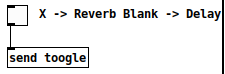
\includegraphics[width=0.3\textwidth]{figuras/fig46.png}
        \caption{botão de seleção de efeito no \textit{PureData}}
        \label{fig46}
    \end{figure}

    O botão \textit{slider} visa alterar os parâmetros internos de cada efeito. Os valores variam de 0 a 1. O botão se encontra na Figura \ref{fig47}.

    \begin{figure}[h]
        \centering
        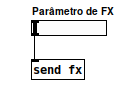
\includegraphics[width=0.2\textwidth]{figuras/fig47.png}
        \caption{botão de quantidade de efeito no \textit{PureData}}
        \label{fig47}
    \end{figure}

    Cada efeito utiliza o parâmetro \textit{fx} advindo do botão \textit{slider} e realiza uma adaptação para o seu parâmetro. No caso do \textit{reverb}, o valor de \textit{fx} é multiplicado por 100 e esse valro se torna a quantidade de dB que permanecerá na música após 1s. Para o \textit{delay}, esse valor é multiplicado por 1000 e se transforma no intervalo de tempo em ms da música que permanecerá no efeito.

    A lógica que permeia a seleção do efeito, encontra-se na Figura \ref{fig48}. Os comandos \texttt{receive\textasciitilde\ fx} são responsáveis por inserirem os efeitos como entrada. Cada volume do efeito é multiplicado pelo valor do \texttt{toogle}; um deles é multiplicado pelo valor atual enquanto o outro é multiplicado pelo inverso, de forma que o botão \texttt{toogle} funciona como um alternador para selecionar os efeitos. 

    \begin{figure}[h]
        \centering
        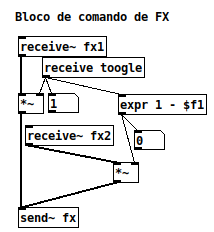
\includegraphics[width=0.3\textwidth]{figuras/fig48.png}
        \caption{botão de seleção de efeito no \textit{PureData}}
        \label{fig48}
    \end{figure}

    Nesse sistema, o volume do efeito é regido de forma automática em função da posição do botão central, ou seja, pelas frequências de corte. Na Figura \ref{fig49} é possível ver a variação do volume do efeito em função da frequência central.

    \begin{figure}[h]
        \centering
        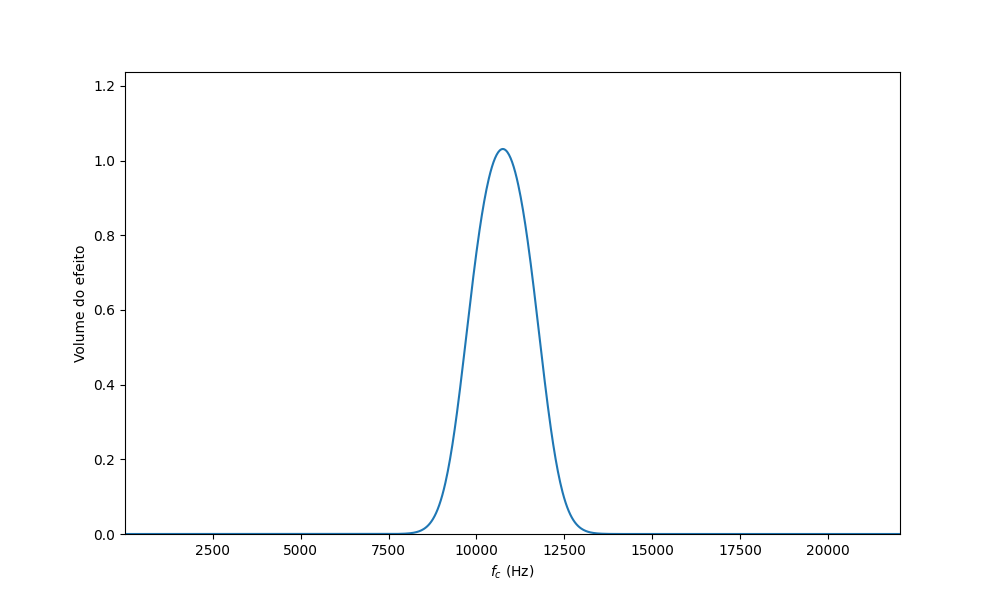
\includegraphics[width=0.9\textwidth]{figuras/fig49.png}
        \caption{variação do volume dos efeitos no \textit{PureData}}
        \label{fig49}
    \end{figure}

    No \textit{PureData}, o bloco de automação de volume de efeitos é realizado utilizando as operações presentes na Figura \ref{fig50}.

    \begin{figure}[h]
        \centering
        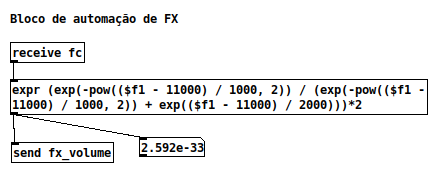
\includegraphics[width=0.6\textwidth]{figuras/fig50.png}
        \caption{implementação da variação do volume dos efeitos no \textit{PureData}}
        \label{fig50}
    \end{figure}

    Ao final, o sinal dos efeitos é multiplicado pelo volume dos efeitos, e, posteriormente, somado ao sinal das filtragens, dando origem ao sinal de saída. Esse sinal é processado por um bloco de conversão de sinal digital em analógico e enfim foi reproduzido. Esse bloco de soma de sinais está representado na Figura \ref{fig51}.

    \begin{figure}[h]
        \centering
        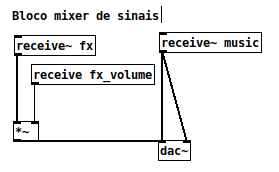
\includegraphics[width=0.3\textwidth]{figuras/fig51.png}
        \caption{soma de sinais filtrado e de efeitos no \textit{PureData}}
        \label{fig51}
    \end{figure}

    \section{Proposta de Implementação}

    \subsection{Implementação em Hardware}

    Texto geral sobre a implementação em hardware percorrendo todos pontos abaixo

    \paragraph{Conectores}
    Para a aquisição dos sinais de áudio, o \textit{mixer} contará com conectores RCA devido à padronização imposta pela indústria e pela facilidade de se ter cabos e entradas desse tipo, Figura \ref{fig22}.

    Dessa forma, dois RCAs serão utilizados para cada canal, sendo assim: 4 RCAs para entrada e 2 RCAs para a saída, totalizando 6 RCAs.

    \paragraph{Botões}

    A interação com o usuário é necessária para a obtenção de parâmetros como frequência de corte, quantidade de efeitos e a seleção do efeito desejado. Para isso, dois \textit{sliders} serão utilizados e uma chave de duas posições, respectivamente. 

    Os \textit{sliders} em si possuem um potenciômetro. Dessa forma, são alimentados por uma tensão e sua posição é obtida através de uma tensão de saída, que é proporcional à tensão de entrada. 

    [INSERIR FIGURA DE SLIDER]

    Em contrapartida, a chave de duas posições gera dois níveis possíveis de tensões, tensão nula ou de alimentação. Cada nível deve se relacionar a um efeito desejado.

    [INSERIR FIGURA DE CHAVE]

    \paragraph{Conversão AD}

    A conversão analógica digital é essencial para que os parâmetros necessários para qu

    
    \paragraph{Protocolos de Comunicação}
    \paragraph{Unidades de Processamento}
    \paragraph{Conversão DA}
    
    
    \subsection{Implementação em Software}
    
    \begin{itemize}
        \item \textbf{Linguagem e Estrutura}
        \begin{itemize}
            \item Descrição da linguagem de programação escolhida (e.g., Python, C++).
            \item Estrutura do código e divisão em módulos/funções.
            \item Abordagem de desenvolvimento (e.g., desenvolvimento ágil, incremental).
        \end{itemize}
    \end{itemize}
    
    \subsection{Integração entre Hardware e Software}
    
    \begin{itemize}
        \item \textbf{Protocolo de Comunicação}
        \begin{itemize}
            \item Descrição dos protocolos de comunicação entre hardware e software (e.g., I2C, SPI, UART, Ethernet).
            \item Mapeamento das funções de software para controlar e receber dados do hardware.
            \item Sincronização e temporização entre o hardware e software.
            \item Gerenciamento de erros e contingências na comunicação.
        \end{itemize}
    \end{itemize}
    
    \subsection{Protótipo de Interface de Usuário}
    
    \begin{itemize}
        \item \textbf{Design da Interface}
        \begin{itemize}
            \item Especificação das telas e controles na interface de usuário.
            \item Ferramentas e frameworks utilizados para o desenvolvimento da interface.
        \end{itemize}
        
        \item \textbf{Interatividade}
        \begin{itemize}
            \item Como os usuários interagem com o sistema.
            \item Feedback visual e sonoro para o usuário.
        \end{itemize}
    \end{itemize}